\documentclass[12pt]{book}

\usepackage{amssymb}
\usepackage{amsmath}
\usepackage{amsthm}
\usepackage{amsfonts}
\usepackage[spanish]{babel}
\usepackage[utf8]{inputenc}
\usepackage[T1]{fontenc}
\usepackage{graphicx}
\usepackage[figuresright]{rotating}
\usepackage{subfigure}
\usepackage{epstopdf}
\usepackage{float}
\usepackage{natbib}
\usepackage[skip=10pt,labelfont=bf,labelsep=period]{caption}
\usepackage[paperwidth=215mm,paperheight=280mm,left=40mm,top=40mm,textwidth=150mm,textheight=215mm]{geometry} 
\usepackage{fancybox}
\usepackage{fancyhdr}
\usepackage{enumerate}
\usepackage{url} 
\usepackage{newtxtext,newtxmath}
\usepackage{bm}

\theoremstyle{definition}
\newtheorem{theorem}{Teorema}[chapter]
\newtheorem{example}[theorem]{Ejemplo}
\newtheorem{proposition}[theorem]{Proposición}
\newtheorem{definition}[theorem]{Definición}
\newtheorem{Lem}[theorem]{Lema}
\newtheorem{Cor}[theorem]{Corolario}
\newtheorem{remark}[theorem]{Observación}
\newtheorem{note}[theorem]{Nota}
\DeclareMathOperator{\sign}{sign}
\DeclareMathOperator*{\argmax}{\arg\,\max}
\usepackage{mathtools}
\newcommand{\Op}[3]{\prescript{}{#2}{#1}^{#3}_{t}}
\newcommand{\OpFull}[5]{\prescript{#1}{#2}{#3}^{#4}_{#5}}
\spanishdecimal{.}

%% Comandos basicos en el texto
%% ==================================================================
\newcommand{\set}[2]{\{#1\nonscript\;\vert\allowbreak\nonscript\:\mathopen{}#2\}}
\usepackage{dsfont}

\begin{document}
\begin{titlepage}

	\vfill

	{\LARGE Trabajo en teoría de Gráficas}\\[2cm]

	\vfill
\end{titlepage}
\section*{Definiciones}
En este trabajo se consideran gráficas simples, finitas, sin lazos.
\begin{definition}
Una gráfica $G$ consta de dos conjuntos $G=(V,E)$, donde $V$ es un conjunto cualquiera y $E\subset \set{\left\{u,v\right\}\subset V}{u\neq v}$. El conjunto $V$ o $V(G)$ es llamado conjunto de vértices de la gráfica $G$. Los elementos de $E$ o $E(G)$ se llaman aristas de la gráfica $G$.
\end{definition}

\begin{definition}
Sea $G=(V,E)$ una gráfica. Si $u,v\in V(G)$ son tal que $\left\{u,v\right\}\in E(G)$, decimos que $u$ y $v$ son adyacentes. Se denota tal adyacencia por $u\sim v$.
\end{definition}

\begin{definition}
Sea $G$ una gráfica. Una subgráfica de $G$ es una gráfica $H$ tal que $V(H)\subset V(G)$ y $E(H)\subset E(G)$.
\end{definition}

\begin{definition}
Sea $G$ una gráfica y $H$ una subgráfica de $G$. $H$ es una subgráfica inducida si para todo $u,v\in V(H)$ tales que $u\sim v$ en $G$ entonces $u\sim v$ en $H$.
\end{definition}

Se entiende que una subgráfica completa $H_n$ tiene cada par de sus $n$ vértices adyacentes. Dicha gráfica completa es maximal si no existe otro vértice en la gráfica tal que forme una completa más grande. Lo anterior da paso a la siguiente definición.

\begin{definition}[\citealt{Harary:1969}]
Un clan de $G$ es una subgráfica completa maximal. 
\end{definition}

\begin{definition}[\citealt{Roberts:1971}]
Dado $G$ una gráfica, sean $C_1, C_2, \dots, C_n $ sus clanes. Definimos $H'$ mediante $ V(H') = \{C_1, C_2, \dots, C_n\}$ y $\left\{C_i, C_j\right\}\in E(H')$ si y solo si $i \neq j$ y $C_i \cap C_j \neq \emptyset$.  
Entonces, llamamos a $H'$ como la gráfica de clanes de $G$ y escribimos $H'=K(G)$.
\end{definition}

\begin{definition}[\citealt{Alcon:2006}]
Sea $G$ una gráfica y $v \in V(G)$. Como es habitual, $G-v$ denota la gráfica inducida por $V(G)\setminus \{v\}$.  

El vértice $v$ es clan crítico si $K(G)\neq K(G-v)$. Una gráfica $G$ es clan crítica si cada uno de sus vértices es crítico.
\end{definition}



\section*{Resultados}

En el siguiente teorema se consideran las gráficas $G(4,3,3)$, que denota a la gráfica con 4 vértices, 3 aristas, número 3; y la gráfica $G(5,7,1)$, que denota la gráfica de 5 vértices, 7 aristas, número 1. Dichas gráficas son extraídas del apéndice de gráficas en \cite{Harary:1969}.
\begin{theorem}
	Sea $G$ una gráfica clan crítica tal que su gráfica de clanes es $K_3$, entonces $G$ es la gráfica $G(4,3,3)$ ó $G(5,7,1)$.
\end{theorem}
\begin{proof}
Sea $G$ una gráfica clan crítica tal que $K(G)=K_3$. Al ser $K(G)=K_3$ entonces existen $C_1,C_2,C_3$ clanes de $G$, representados como los vértices de $K_3$, tal que se intersecan de alguna manera, más aún, cada par de clanes se interseca en al menos un vértice de $G$, es decir
\begin{equation*}
C_i\cap C_j\neq \emptyset, \quad \forall i,j\in\{1,2,3\},\quad i\neq j.
\end{equation*}
Sea $u_1$ el vértice de $G$ en el que se intersecan necesariamente los tres clanes de $G$, es decir $C_1\cap C_2 \cap C_3=\{u_1\}$, veamos que esto es así.

Supongamos que no existe un vértice $u_1$ que pertenezca simultáneamente a los tres clanes, es decir  $C_1\cap C_2 \cap C_3=\emptyset$. Bajo este supuesto, cada intersección $C_i\cap C_j$ contiene al menos un vértice, pero no hay un vértice común a todos. Esto significa que podemos elegir un vértice $v$ en una de estas intersecciones y eliminarlo sin afectar la estructura de $K(G)$ , ya que los otros clanes seguirán intersecándose en otros vértices. Esto contradice la propiedad de clan crítica, pues existiría un vértice cuya eliminación no cambiaría la gráfica de clanes.
Por lo tanto, necesariamente debe existir al menos un vértice $u_1$ tal que
\begin{equation*}
C_1\cap C_2 \cap C_3=\{u_1\}.
\end{equation*}

Para dichas intersecciones, resultan los siguientes casos a considerar.
\begin{itemize}
\item Caso 1. 
Los clanes de $G$ se intersecan únicamente en el vértice $u_1$, es decir $C_1\cap C_2\cap C_3=\left\{u_1\right\}$ y $(C_1\cap C_3)\setminus C_2=\left\{\emptyset\right\}  \text{ y }(C_2\cap C_3)\setminus C_1=\left\{\emptyset\right\}$, como se muestra en la figura~\ref{F1}.

\begin{figure}[!htbp]
	\centering
	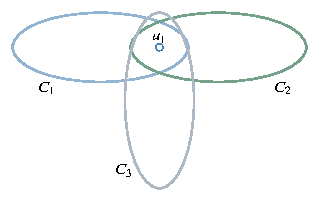
\includegraphics[scale=1.2]{Fig1.pdf}
	\caption{Esquema de los clanes de la gráfica $G$ correspondiente al caso 1.\label{F1}}
\end{figure}

De primera instancia, los tres clanes pueden ser tales que $|C_i|=n$ con $i=1,2,3$, considerando el vértice $u_1$ claramente; sin embargo, de considerar un $n>2$, la gráfica $G$ no cumpliría la condición de ser clan crítica, pues resultaría que $K(G)=K(G-\hat{u})$, para cualquier $\hat{u}\in V(C_i)$ y $\hat{u}\neq u_1$. Por lo tanto cada clan consta únicamente de dos vértices, uno de ellos $u_1$, con lo cual la gráfica $G=G(4,3,3)$, la cual cumple que $K(G)=K_3$.

\item Caso 2.
Existe una intersección dos a dos entre los clanes, de más de un vértice, considerando el vértice $u_1$. Sin pérdida de generalidad, supongamos que el clan $C_3$ interseca al clan $C_1$ en un vértice $u_2\in V(G)$, así como a $C_2$ en un vértice $u_3\in V(G)$, esto es 
\begin{equation*}
\left\{u_2\right\}=(C_1\cap C_3)\setminus C_2 \quad \text{y} \quad \left\{u_3\right\}=(C_2\cap C_3)\setminus C_1.
\end{equation*}
Como se muestra en la figura~\ref{F2}.

\begin{figure}[!htbp]
	\centering
	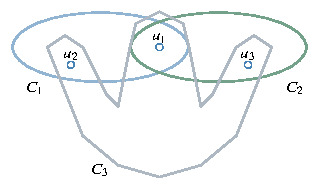
\includegraphics[scale=1.2]{Fig2.pdf}
	\caption{Esquema de los clanes de la gráfica $G$ correspondiente al caso 2.\label{F2}}
\end{figure}

Los clanes $C_1$ y $C_2$ no pueden ser tales que están constituidos únicamente de dos vértices, veamos que esto es así. Supongamos que $|C_1|=2$ y $|C_2|=2$, con lo cual $\left\{\left\{u_2,u_1\right\},\left\{u_1,u_3\right\},\left\{u_2,u_3\right\}\right\}\subset E(G)$, de esta manera, las únicas aristas de $G$ entre los clanes serían aquellas en $C_3$ que conectan $u_1$ con $u_2$ y $u_3$. Sin embargo, en este caso al eliminar cualquier vértice en $C_3$ que no sea $u_1,u_2,u_3$, la gráfica de clanes seguiría siendo $K_3$, lo que contradice la propiedad de $G$ de ser clan crítica. Como los clanes $C_1$ y $C_2$ no pueden tener solo dos vértices, deben tener al menos tres.
Siguiendo este razonamiento, se puede concluir que $|C_1|=|C_2|=|C_3|=3$, lo que da lugar a la gráfica $G=G(5,7,1)$ y es claro que $K(G)=K_3$.


\item Caso 3.
Los clanes de $G$ se intersecan en el vértice $u_1$ y sólo existe otra intersección entre dos de estos clanes. Sin pérdida de generalidad, supongamos que los clanes $C_1$ y $C_3$ se intersecan en un vértice $u_2$ de $G$ y $(C_2\cap C_3)\setminus C_1=\left\{\emptyset\right\}$, como se muestra en la figura~\ref{F3}.

\begin{figure}[!htbp]
	\centering
	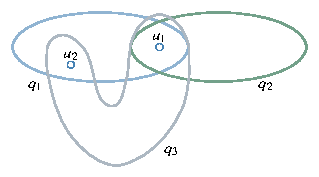
\includegraphics[scale=1.2]{Fig3.pdf}
	\caption{Esquema de los clanes de la gráfica $G$ correspondiente al caso 3.\label{F3}}
\end{figure}

Dado que $G$ es clan crítica, se sigue que la eliminación de cualquier vértice de $G$ cambia la estructura de su gráfica de clanes $K(G)$. Utilizando un argumento similar al del caso anterior, se concluye que $C_1=C_3=K_3$, pues de no ser así, no se satisface la hipótesis de ser $G$ clan crítica. Si alguno de estos clanes tuviera menos de tres vértices, entonces existiría un vértice $\hat{u}$ en $C_1$ ó $C_3$ cuya eliminación no cambiaría la estructura de $K(G)$, lo que contradice la definición de clan crítica.

Sea $u_3\in V(C_3)$ tal que $u_3\neq u_1,u_2$ y que satisface la inclusión $\left\{\left\{u_2,u_1\right\},\left\{u_1,u_3\right\},\left\{u_2,u_3\right\}\right\}\subset E(G)$. El clan $C_2$ debe estar constituido de más de dos vértices, pues de no ser así, consideremos un nuevo vértice $\hat{u}\neq u_1$ en $C_2$, ver figura~\ref{F4}.

\begin{figure}[!htbp]
	\centering
	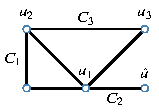
\includegraphics[scale=1.2]{Fig4.pdf}
	\caption{Esquema de los vértices y clanes de la gráfica $G$ correspondiente al caso 3, suponiendo que $C_2$ cuenta únicamente con dos vértices.\label{F4}}
\end{figure}

En tal caso se cumple que $K(G-u_2)=K(G)$, situación que no es válida. Con lo cual $|C_2|>2$ y se consideran los siguientes dos casos.
\begin{itemize}
\item Caso 3.1.
El vértice $u_3\notin V(C_2)$, entonces para todo $\overline{u}\in V(C_2)\setminus\{u_1\}$ se tiene que $K(G-\overline{u})=K(G)$, lo que implica que este caso no es posible, pues la eliminación de cualquier vértice de $C_2$, excepto $u_1$, no provoca un cambio en la estructura de $K_3$, lo que contradice la hipótesis de clan crítica.

\item Caso 3.2.
El vértice $u_3\in V(C_2)$. Este caso se reduce al caso 2, con lo cual $G=G(5,7,1)$ y por lo tanto $K(G)=K_3$.
\end{itemize}
\end{itemize}
Resulta entonces que $G$ es la gráfica $G(4,3,3)$ ó $G(5,7,1)$.
\end{proof}


\bibliography{Ref}
\bibliographystyle{apalike}

\end{document}